\section*{Концептуальный дизайн}
Концептуальный дизайн позволяет рассмотреть создаваемую систему с точки зрения пользователей. На рисунке \ref{fig:idef0-1} отображена контекстная диаграмма верхнего уровня, которая обеспечивает наиболее общее или абстрактное описание работы системы. Данный вид диаграммы позволяет формализовать описание запросов пользователя и ответов системы на них, отобразив её в виде <<чёрного ящика>>.

Для уточнения деталей по операции бронирования, отображённой на диаграмме верхнего уровня, используется дочерняя диаграмма, которая изображена на рисунке \ref{fig:idef0-2}. Она определяет последовательность выполнения операций в системе при обработке запроса клиента. 

\begin{figure}[h!]
	\begin{center}
		{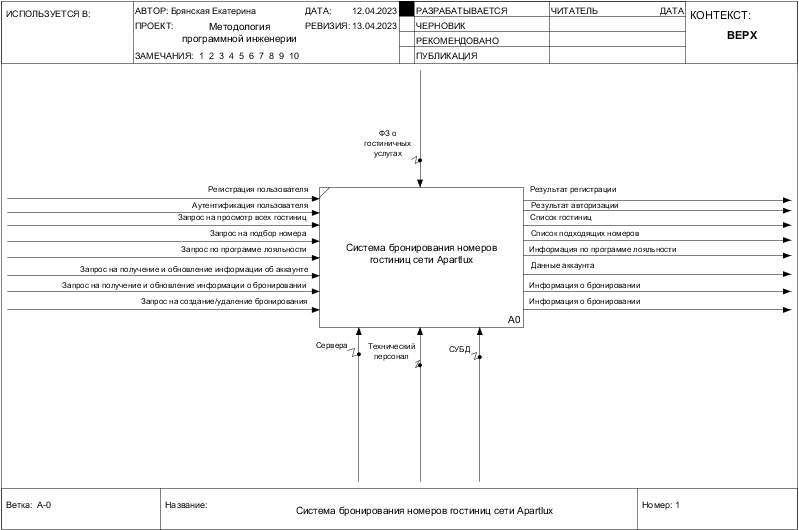
\includegraphics[scale = 0.82, angle=90]{img/idef0/01_A-0.png}}
		\caption{Концептуальная модуль системы в нотации IDEF0.}
		\label{fig:idef0-1}
	\end{center}
\end{figure}

\begin{figure}[h!]
	\begin{center}
		{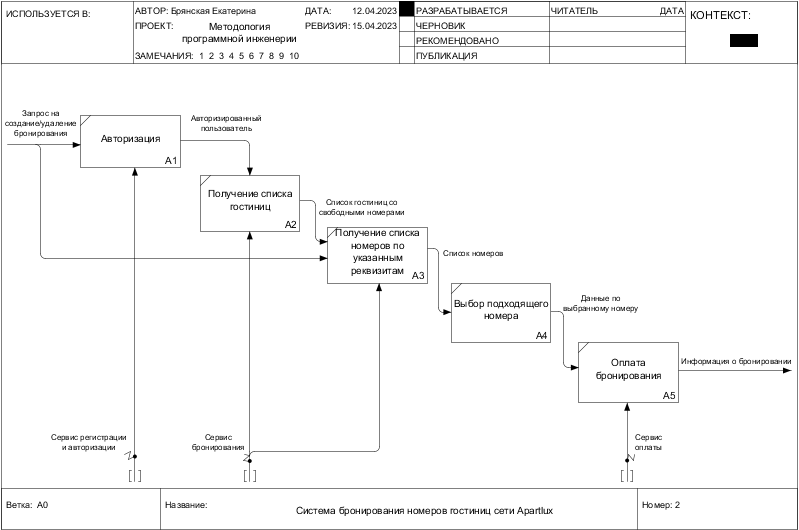
\includegraphics[scale = 0.79, angle=90]{img/idef0/02_A0.png}}
		\caption{Детализированная концептуальная модель системы в нотации IDEF0.}
		\label{fig:idef0-2}
	\end{center}
\end{figure}

\pagebreak

\section*{Сценарии функционирования системы}
\textbf{Регистрация клиента}
\begin{enumerate}
	\item Пользователь нажимает на кнопку <<Зарегистрироваться>> в интерфейсе.
	
	\item Пользователь перенаправляется на страницу, которая содержит поля для заполнения его данных.
	
	\item Пользователь вводит данные в форму и для завершения регистрации нажимает на кнопку <<Готово>>, тем самым подтверждая верность своих данных, а также согласие на их обработку и хранение.
	
	\item Если пользователь с введенным для регистрации логином уже существует, то клиент перенаправляется на страницу ошибки. При успешной регистрации клиент попадает на страницу своего профиля в системе. \\
\end{enumerate}

\textbf{Авторизация клиента}
\begin{enumerate}
	\item Пользователь нажимает на кнопку <<Войти>> в интерфейсе.
	
	\item Пользователь перенаправляется на страницу авторизации, которая содержит поля для заполнения логина и пароля.
	
	\item Пользователь завершает работу с формой авторизации нажатием кнопки <<Готово>>.
	
	\item При обнаружении ошибки в данных, пользователь перенаправляется на страницу ошибки; при совпадении данных с записью в базе данных аккаунтов пользователь получает доступ к системе. \\
\end{enumerate}

\textbf{Бронирование номера}
\begin{enumerate}
	\item Клиент нажимает кнопку <<Бронирование>>.
	
	\item Клиент перенаправляется на страницу, которая содержит список гостиниц.
	
	\item Клиент нажимает на понравившуюся позицию и попадает на страницу доступных для бронирования номеров в выбранной гостинице с разными реквизитами.
	
	\item При необходимости выставляет необходимые параметры фильтров (например, адрес, планировка, диапазон цен и дат), нажимает кнопку <<Применить>>. После этого список обновляется, сверху находятся предложения, наиболее соответствующие желанию клиента.
	
	\item Клиент нажимает кнопку <<Оформить бронирование>> напротив нужного номера, на экране появляется всплывающее окно, дублирующее его атрибуты.
	
	\item Клиент нажимает кнопку <<Готово>>, выражая своё согласие на оформление бронирования, и перенаправляется на страницу оплаты, где вводит реквизиты карты и код подтверждения. В случае успешной операции придёт смс- и email-оповещения.
	
	\item Если клиент не хочет оформлять бронь, он нажимает на кнопку выхода -- крестик, всплывающее окно пропадает. \\
\end{enumerate}

\section*{Диаграммы прецендентов}
В системе выделены три роли: Пользователь, Клиент, Администратор. На рисунках \ref{fig:use-case-user}-\ref{fig:use-case-admin} представлены диаграммы прецедентов для каждой из ролей. В таблицах \ref{tbl:scenario-1}-\ref{tbl:scenario-2} описаны сценарии функционирования наиболее значимых прецедентов.  

\begin{figure}[h]
	\begin{center}
		{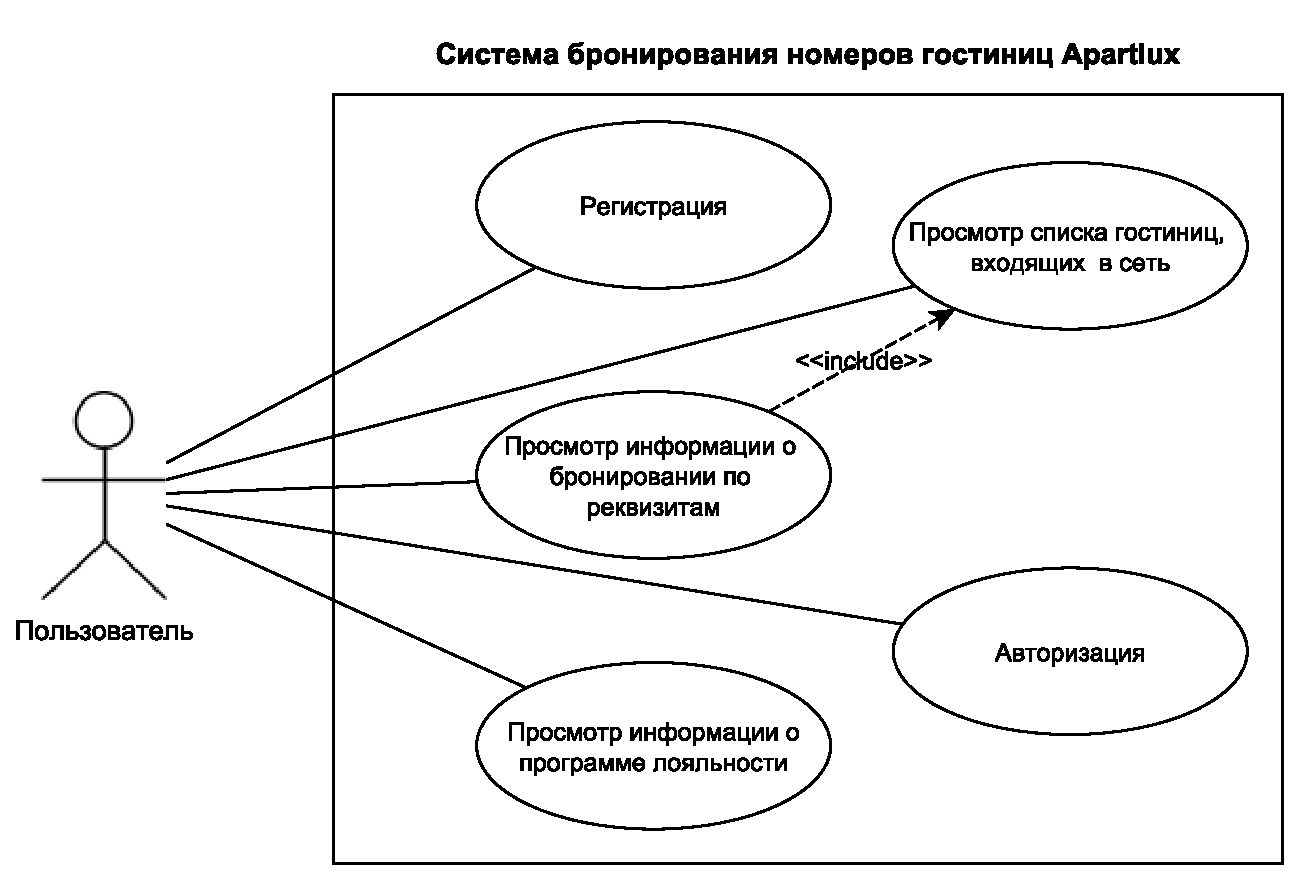
\includegraphics[scale = 0.6]{img/use-case/user.pdf}}
		\caption{Диаграмма прецедентов с точки зрения пользователя.}
		\label{fig:use-case-user}
	\end{center}
\end{figure}

\pagebreak

\begin{longtable}{| p{6cm} | p{10cm} |}
	\caption{Спецификация сценария регистрации}
	\label{tbl:scenario-1} \\
	\hline
	
	\multicolumn{2}{|c|}{\textbf{Нормальный ход сценария}} \\
	\hline
	
	\textbf{Действия актера} & \textbf{Отклик системы} \\
	\hline
	\endfirsthead
	
	\hline
	\textbf{Действия актера} & \textbf{Отклик системы} \\
	\hline
	\endhead
	
	\hline
	\multicolumn{2}{c}{\textit{Продолжение на следующей странице}}
	\endfoot
	\hline
	\endlastfoot
	
	Регистрация
	&
	Система предоставляет актеру форму для регистрации, в которой нужно заполнить ФИО, дату рождения, логин, пароль, номер телефона, электронную почту \\
	\hline
	
	Актер заполняет форму и даёт согласие на обработку данных
	&
	Данные актера регистрируются в системе \\
	\hline
	
	\multicolumn{2}{|c|}{\textbf{Альтернативный ход сценария}} \\
	\hline
	
	Регистрация
	&
	Система предоставляет актеру форму для регистрации, в которой нужно заполнить ФИО, дату рождения, логин, пароль, номер телефона, электронную почту \\
	\hline
	
	Актер не заполняет форму или не даёт согласие на обработку данных
	&
	Актер не заносится в клиентскую базу данных
\end{longtable}

\begin{figure}[h]
	\begin{center}
		{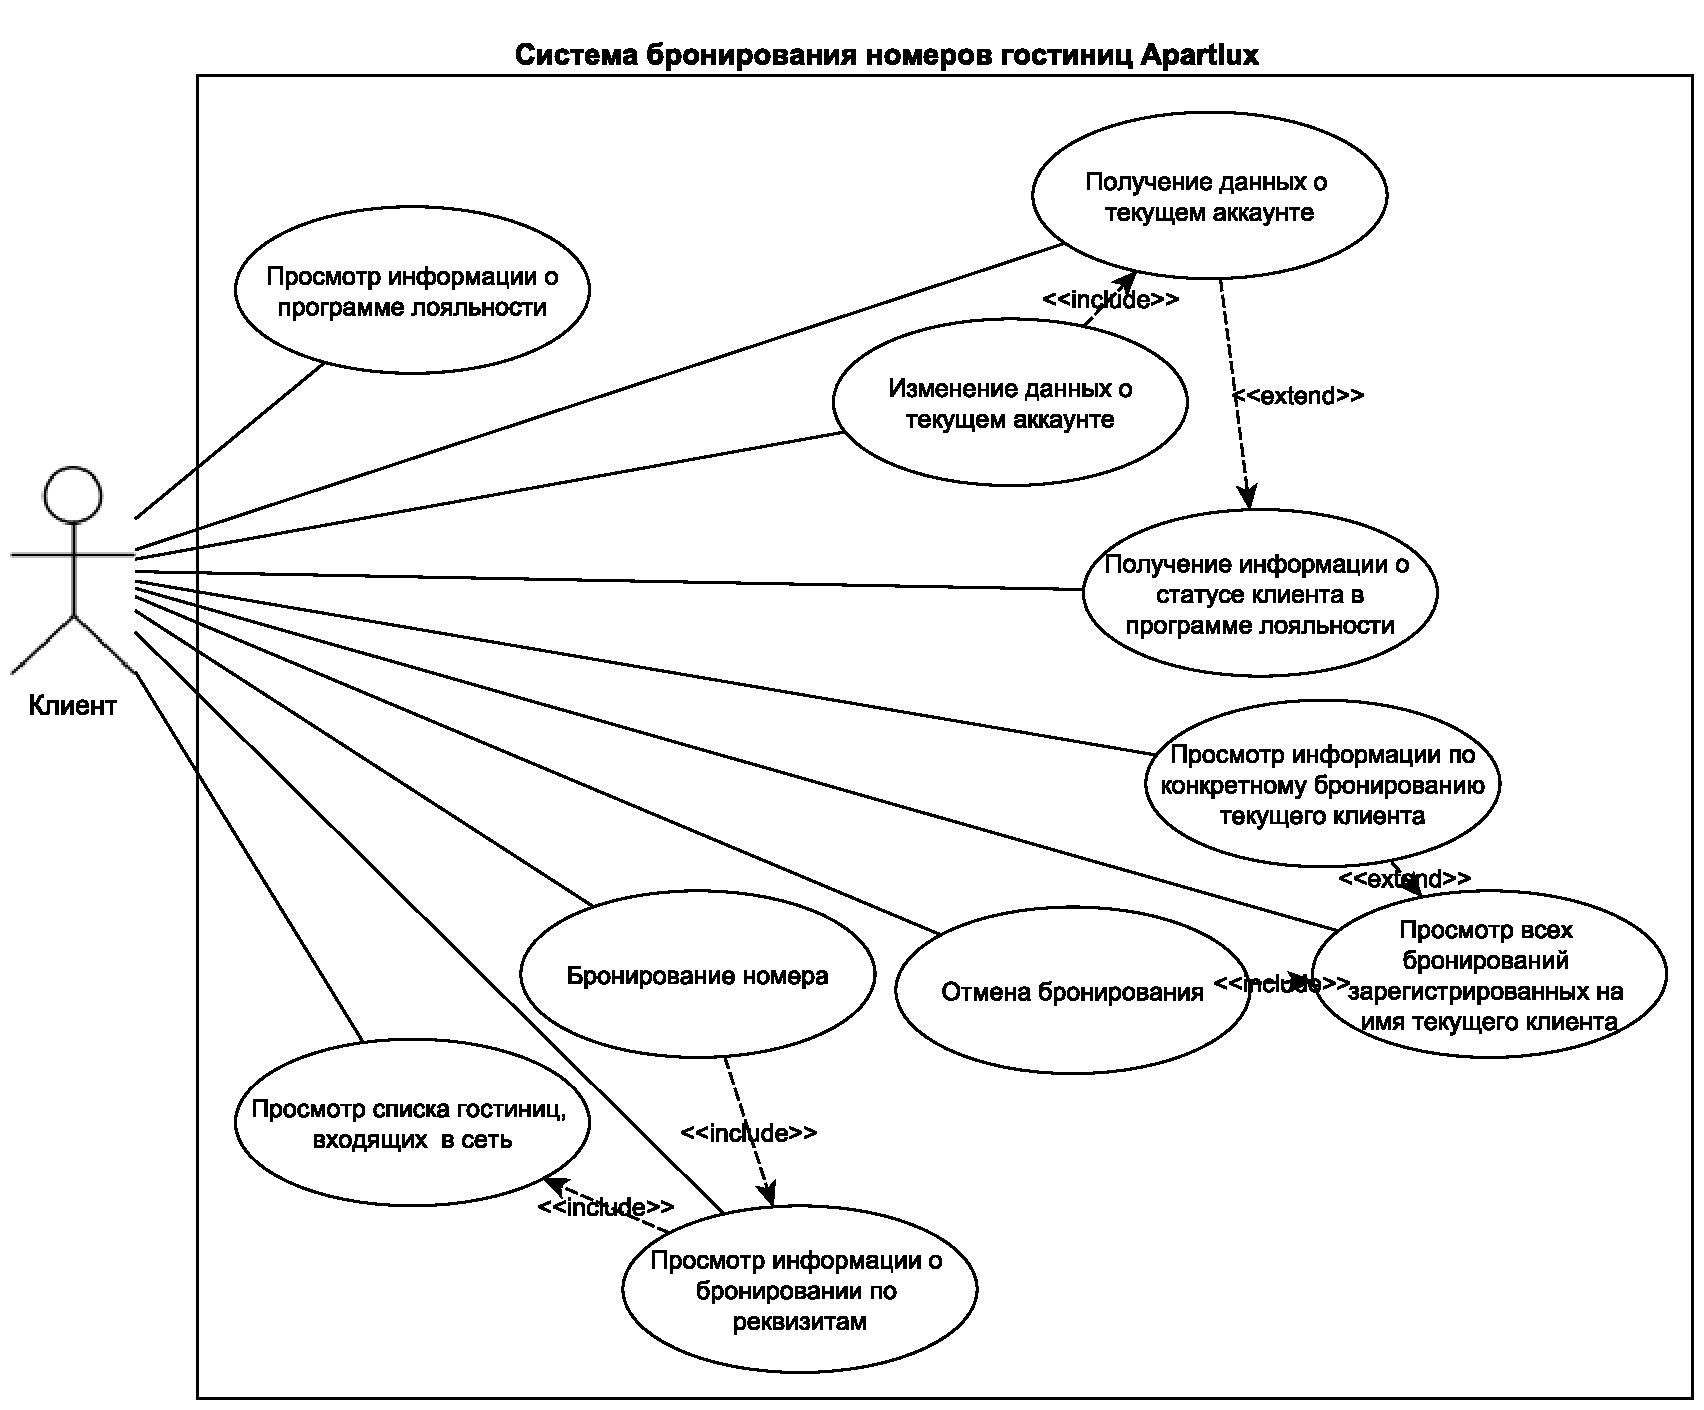
\includegraphics[scale = 0.56]{img/use-case/client.pdf}}
		\caption{Диаграмма прецедентов с точки зрения клиента.}
		\label{fig:use-case-client}
	\end{center}
\end{figure}

\begin{longtable}{| p{6cm} | p{10cm} |}
	\caption{Спецификация сценария бронирования}
	\label{tbl:scenario-2} \\
	\hline
	
	\multicolumn{2}{|c|}{\textbf{Нормальный ход сценария}} \\
	\hline
	
	\textbf{Действия актера} & \textbf{Отклик системы} \\
	\hline
	\endfirsthead
	
	\hline
	\textbf{Действия актера} & \textbf{Отклик системы} \\
	\hline
	\endhead
	
	\hline
	\multicolumn{2}{c}{\textit{Продолжение на следующей странице}}
	\endfoot
	\hline
	\endlastfoot
	
	Просмотр списка гостиниц, входящих в сеть
	&
	Система предоставляет актеру список гостиниц, которые входят в состав сети Apartlux и предоставляющих свободные для бронирования номера \\
	\hline
	
	Просмотр информации о возможном бронировании по заданным реквизитам (дата, цена, количество мест и т.д.)
	&
	Система предоставляет актеру ранжированный список номеров, наиболее подходящих под параметры фильтрации, указанные клиентом \\
	\hline
	
	Бронирование
	&
	Система перенаправляет актера на страницу оплаты, после успешной транзакции фиксирует выбранный номер за клиентом \\
	\hline
	
	\multicolumn{2}{|c|}{\textbf{Альтернативный ход сценария}} \\
	\hline
	
	Просмотр списка гостиниц, входящих в сеть
	&
	Система предоставляет актеру список гостиниц, которые входят в состав сети Apartlux и предоставляющих свободные для бронирования номера \\
	\hline
	
	Актер не выбирает ни одну гостиницу из предоставленных
	&
	\\
	\hline
	
	\multicolumn{2}{|c|}{\textbf{Альтернативный ход сценария}} \\
	\hline
	
	Просмотр списка гостиниц, входящих в сеть
	&
	Система предоставляет актеру список гостиниц, которые входят в состав сети Apartlux и предоставляющих свободные для бронирования номера \\
	\hline
	
	Просмотр информации о возможном бронировании по заданным реквизитам (дата, цена, количество мест и т.д.)
	&
	Система предоставляет актеру ранжированный список номеров, наиболее подходящих под параметры фильтрации, указанные клиентом \\
	\hline
	
	Актер не выбирает ни одного номера и либо завершает работу с системой, либо осуществляет поиск дальше
	&
	\\
	\hline
	
	\multicolumn{2}{|c|}{\textbf{Альтернативный ход сценария}} \\
	\hline
	
	Просмотр списка гостиниц, входящих в сеть
	&
	Система предоставляет актеру список гостиниц, которые входят в состав сети Apartlux и предоставляющих свободные для бронирования номера \\
	\hline
	
	Просмотр информации о возможном бронировании по заданным реквизитам (дата, цена, количество мест и т.д.)
	&
	Система предоставляет актеру ранжированный список номеров, наиболее подходящих под параметры фильтрации, указанные клиентом \\
	\hline
	
	Бронирование (транзакция завершилась с ошибкой)
	&
	Система перенаправляет актера на страницу оплаты, из-за проблем с платёжной операцией актеру предлагается повторить попытку, номер на актера не регистрируется
\end{longtable}

\begin{figure}[h]
	\begin{center}
		{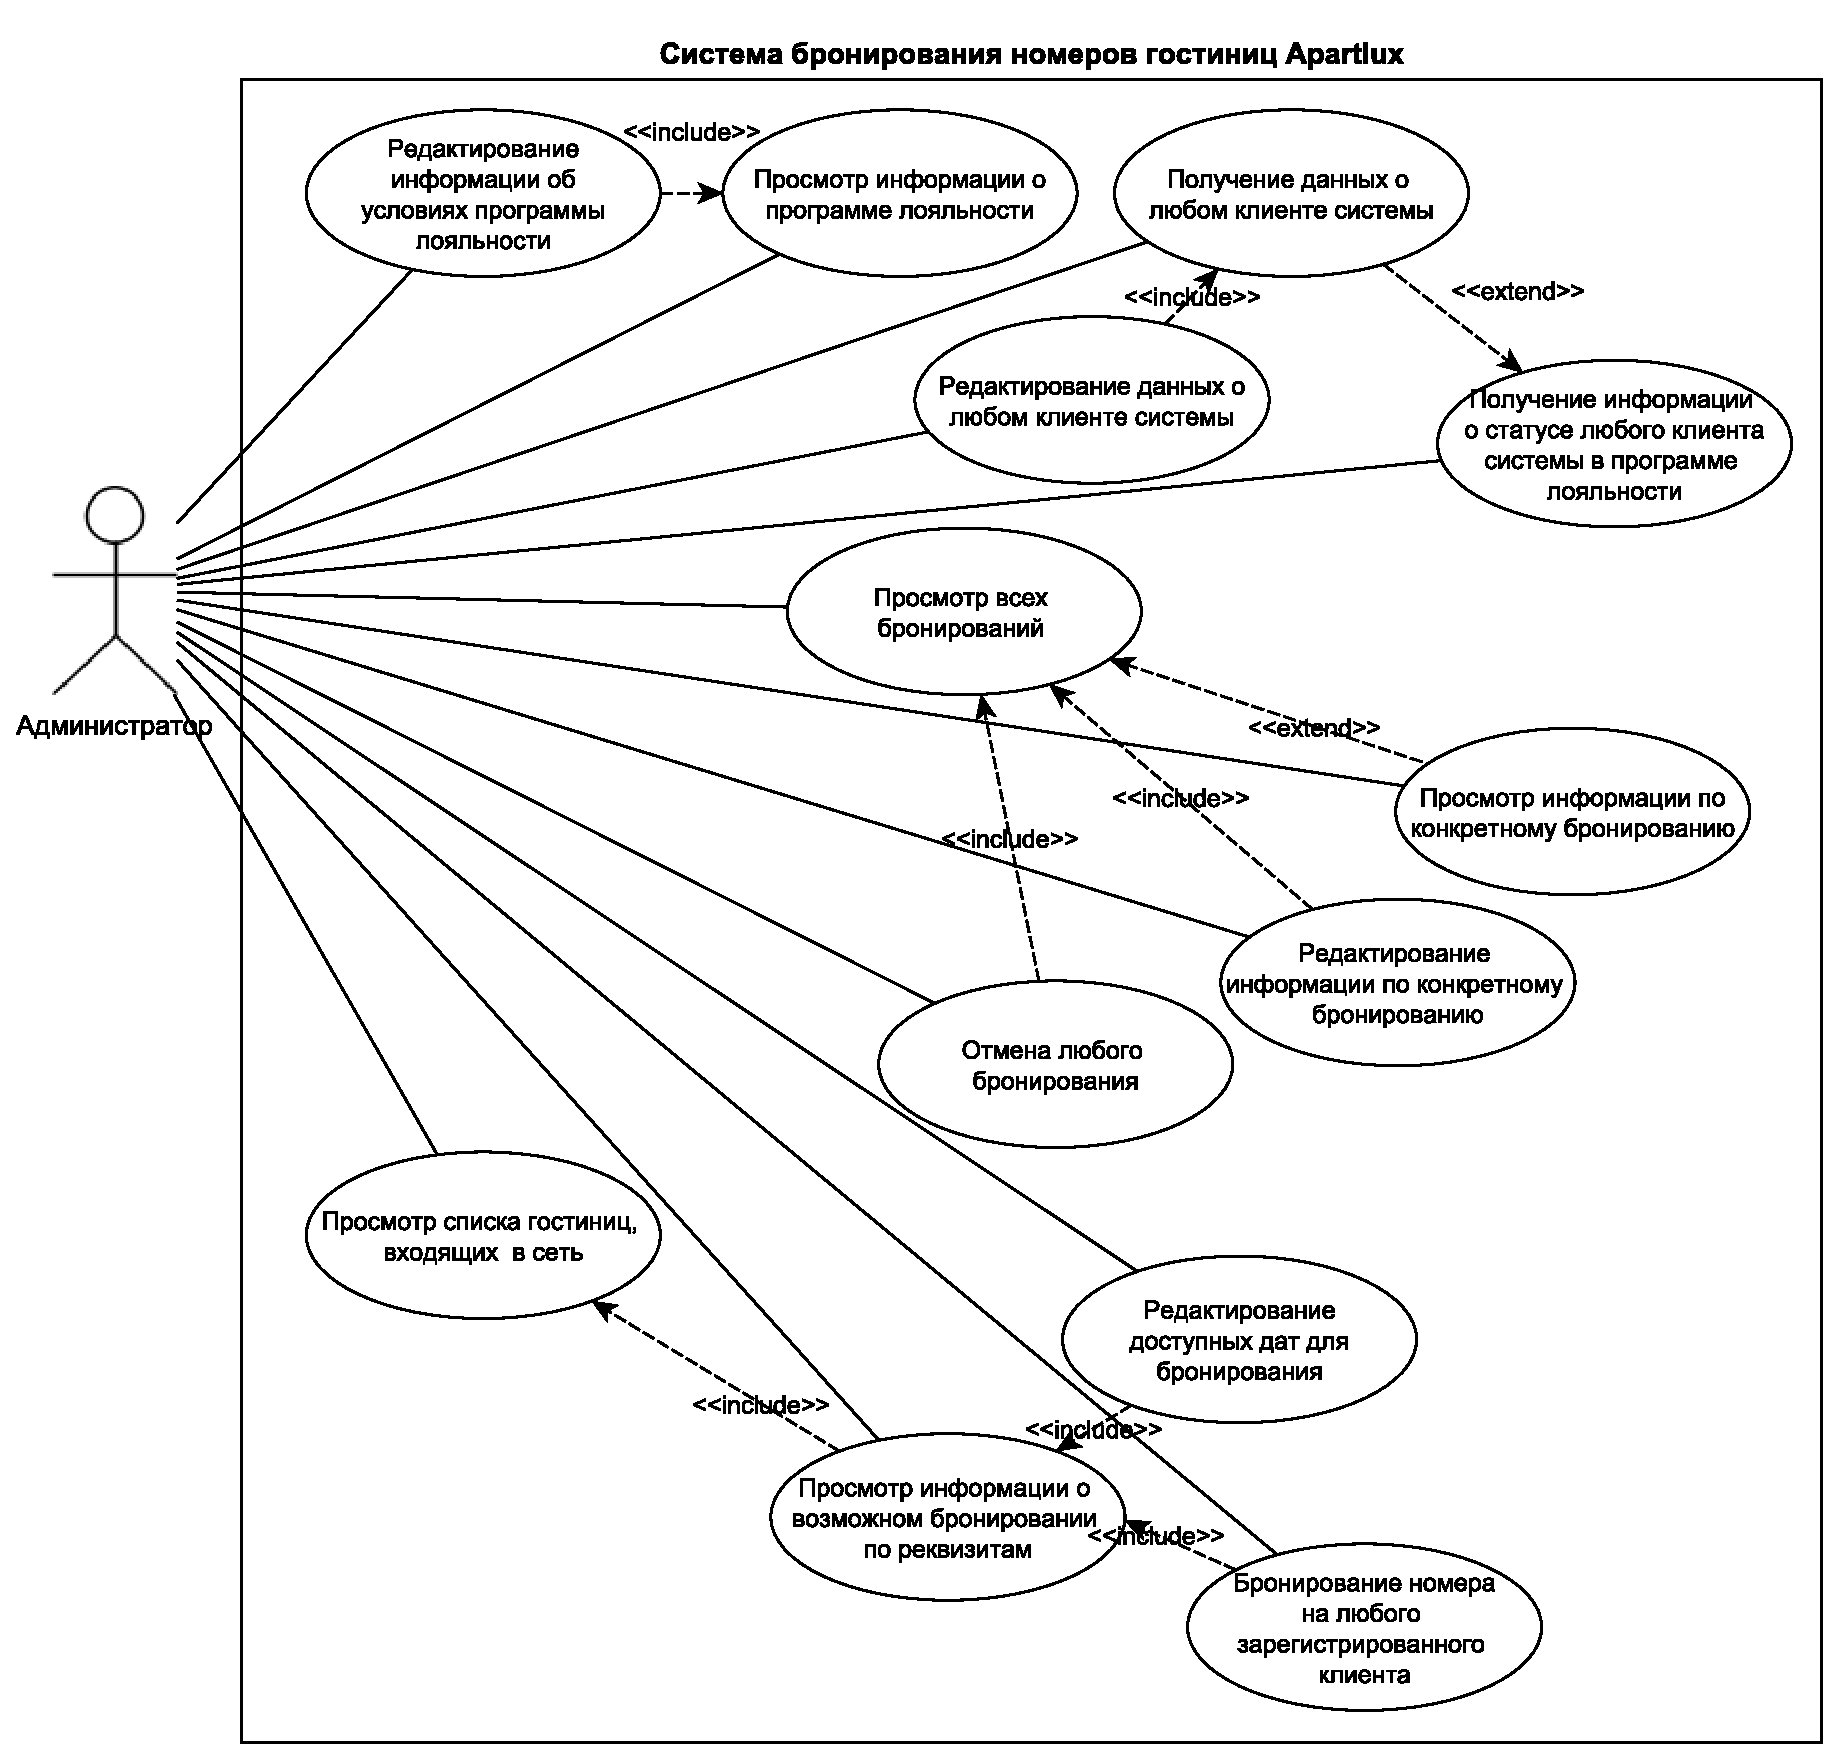
\includegraphics[scale = 0.54]{img/use-case/admin.pdf}}
		\caption{Диаграмма прецедентов с точки зрения администратора.}
		\label{fig:use-case-admin}
	\end{center}
\end{figure}

\pagebreak